\section{Simulation-Based Validation}
\label{sec:validation}

Due to airspace constraints, no powered flight testing was conducted. System behavior was evaluated
using a physics-based simulation incorporating rigid-body rotational dynamics, thrust vector geometry,
actuator limits, and PID control laws.

% -----------------------------------------------------------------------
\subsection{Overview of Simulation Objectives}
\label{subsec:sim_objectives}

To evaluate the performance and robustness of the thrust vector control system in the absence of powered flight testing, a comprehensive set of physics-based simulations was developed in Python. The simulation integrates rigid-body rotational dynamics using a fourth-order Runge-Kutta (RK4) scheme at a 1 ms time step, with the Estes E12-4 thrust curve represented by NAR-certified data points interpolated via numpy. The control architecture, which includes the discrete-time PD controller (the integral term is disabled for this simulation, $K_i = 0$, per Section 3.1), Kalman filter, and servo rate limiting, runs at 150 Hz within the simulation loop to match the intended flight computer update rate. It is important to note that the simulations assume a rigid airframe, constant atmospheric conditions, and no launch rail dynamics. These simplifications are discussed further in Section \ref{subsec:sim_discussion}.


% -----------------------------------------------------------------------
\subsection{Motor Thrust Profile}
\label{subsec:thrust_profile}

Before examining control system behavior, it is useful to understand the propulsive input driving
the simulation. Figure~\ref{fig:thrust_curve} shows the NAR-certified thrust curve for the Estes
E12-4 motor, interpolated from published data points sourced from ThrustCurve.org
\cite{nar_thrustcurve}. The motor produces a sharp peak of 33.0~N at approximately $t = 0.29$~s,
followed by a gradual decay to a plateau of roughly 9.5~N before burnout at 2.44~s, with a mean
thrust of 11.12~N. This time-varying thrust profile is significant for control system design:
available corrective torque is directly proportional to instantaneous thrust, meaning control
authority is highest immediately after ignition and diminishes steadily toward burnout.

\begin{figure}[ht]
    \centering
    % IMAGE NEEDED: Export from Python as sections/fig_e12_thrust_curve.png
    % (NAR certified data points + interpolated curve, mean thrust + burnout lines labelled)
    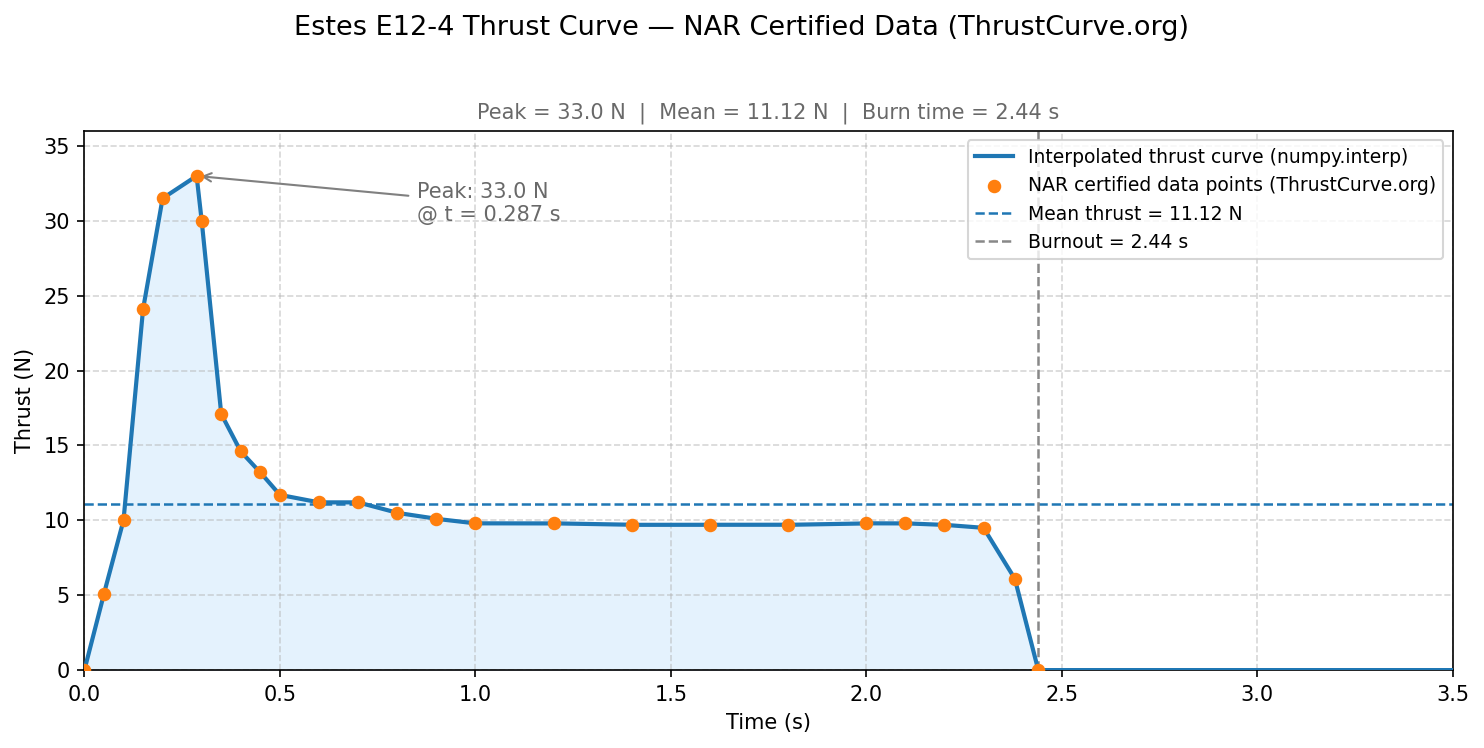
\includegraphics[width=0.85\linewidth]{figures/fig01_thrust_curve.png}
    \caption{Estes E12-4 Thrust Curve --- NAR Certified Data (ThrustCurve.org).
             Peak = 33.0~N at $t = 0.29$~s, Mean = 11.12~N, Burn time = 2.44~s.}
    \label{fig:thrust_curve}
\end{figure}

\FloatBarrier

% -----------------------------------------------------------------------
\subsection{Baseline Closed-Loop Response}
\label{subsec:baseline_response}

Figure~\ref{fig:baseline_response} shows the baseline closed-loop attitude response to a 5\degree{}
initial pitch offset, representing a realistic launch tip-off disturbance. The top panel shows that
the true pitch angle is driven back toward vertical within approximately 0.3~seconds of ignition,
with the Kalman filter estimate tracking closely during powered flight. The middle panel shows the
corresponding angular rate, which peaks near $-45~\mathrm{deg/s}$ immediately after correction
begins before decaying smoothly as the controller damps rotational motion. The bottom panel shows
gimbal deflection, which briefly approaches the mechanical limit at the onset of correction before
reducing to small oscillatory commands as the vehicle settles. After motor burnout at 2.44 s, the control loop is disabled and, with the vehicle in near-freefall, the accelerometer no longer senses a usable gravity reference; the Kalman estimate therefore drifts based on gyroscope integration alone. This is distinct from the roll-axis heading drift discussed in Appendix~\ref{subsubsec:sensor_limits}, which is a magnetometer-related limitation that applies specifically during powered flight.

\begin{figure}[ht]
    \centering
    % IMAGE NEEDED: Export from Python as sections/fig_baseline_response.png
    % (3-panel: pitch angle with Kalman estimate, angular rate, gimbal deflection vs. time;
    %  motor burn window shaded, gyro drift post-burnout annotated)
    
\includegraphics[width=0.90\linewidth]{figures/fig02_baseline_response.png}
    \caption{Attitude Stabilisation Using TVC --- Baseline Closed-Loop Response.
             Top: pitch angle (true vs.\ Kalman estimate). Middle: angular rate.
             Bottom: gimbal deflection with $\pm$10\degree{} mechanical limits shown.
             Motor burn window shaded; post-burnout gyroscopic drift annotated.}
    \label{fig:baseline_response}
\end{figure}

\FloatBarrier

% -----------------------------------------------------------------------
\subsection{Open-Loop vs.\ Closed-Loop Comparison}
\label{subsec:open_vs_closed}

Figure~\ref{fig:open_vs_closed} provides the most direct argument for the necessity of active
thrust vector control in this finless configuration. Starting from the same 5\degree{} initial offset, the open-loop case\textemdash representing a rocket with no active stabilization\textemdash shows no tendency to return toward vertical. Because the vehicle is aerodynamically unstable in this finless configuration (Section 2.5), there is no restoring moment to correct the deviation; at the relatively low dynamic pressures and short burn duration modeled here, the destabilizing aerodynamic moment is not large enough to produce visible growth of the tilt angle over the burn window shown, but the same lack of a restoring moment means that, given more time, a larger initial disturbance, or higher dynamic pressure, this deviation would diverge rather than decay. The closed-loop case corrects the same disturbance within approximately 0.3 seconds and maintains near-zero pitch angle through burnout. This contrast illustrates that passive stability is entirely absent in this design, and that the PID-Kalman control architecture is solely responsible for maintaining a stable trajectory.

\begin{figure}[ht]
    \centering
    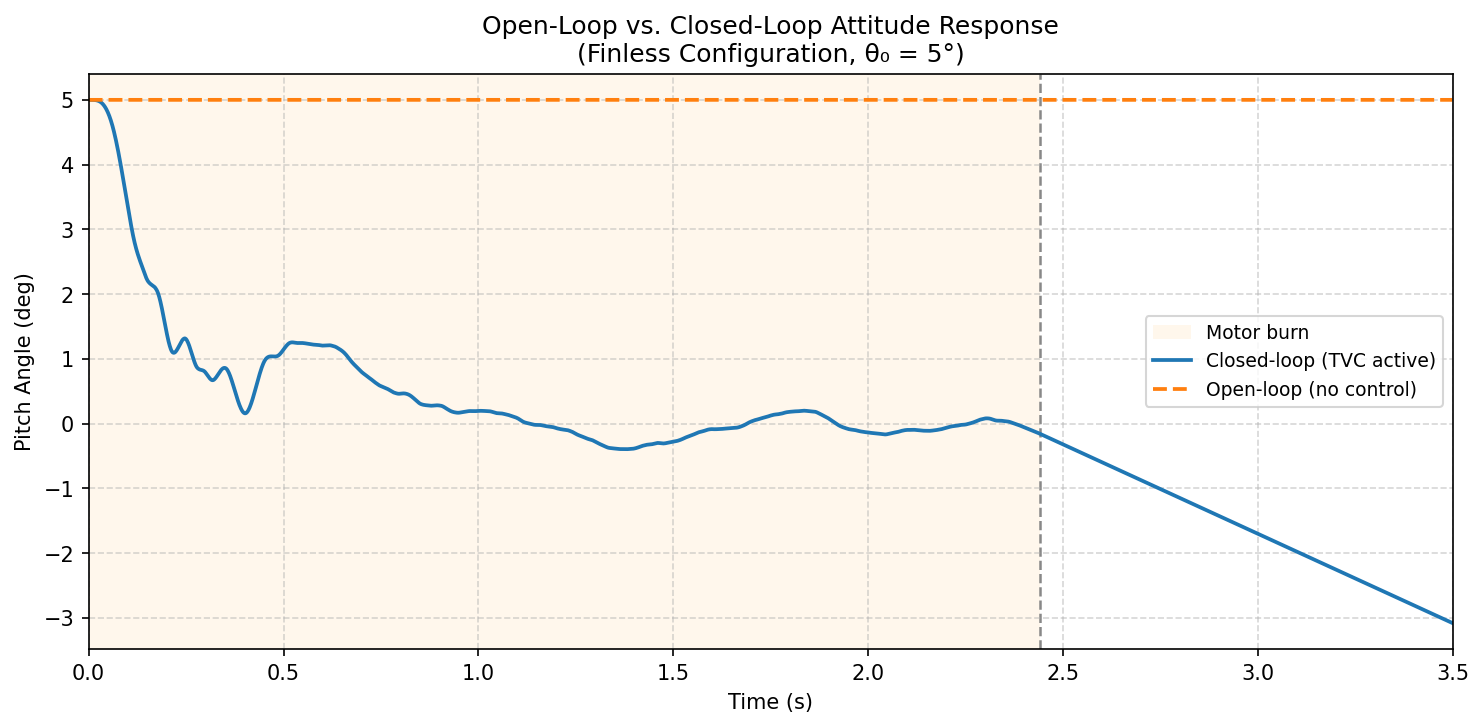
\includegraphics[width=0.85\linewidth]{figures/fig03_open_vs_closed.png}
    \caption{Open-Loop vs.\ Closed-Loop Attitude Response (Finless Configuration,
             $\theta_0 = 5\degree$). Without active control, the initial offset persists
             throughout the burn. Closed-loop TVC corrects the disturbance within $\sim$0.3~s.}
    \label{fig:open_vs_closed}
\end{figure}

\FloatBarrier

% -----------------------------------------------------------------------
\subsection{Disturbance Rejection Response}
\label{subsec:disturbance}

Figure~\ref{fig:disturbance} evaluates the system's ability to reject a mid-flight external
disturbance. A torque impulse of 0.12~N$\cdot$m applied for 50~ms at $t = 0.6$~s simulates
the effect of a wind gust or aerodynamic transient during powered ascent. The disturbance produces
a peak angular deviation of approximately 1.3\degree{} before the controller arrests the motion and
returns the vehicle toward its nominal trajectory. Recovery is stable and completes within
0.4~seconds. This result suggests the system has reasonable tolerance to aerodynamic disturbances
within the modeled range.

\begin{figure}[ht]
    \centering
    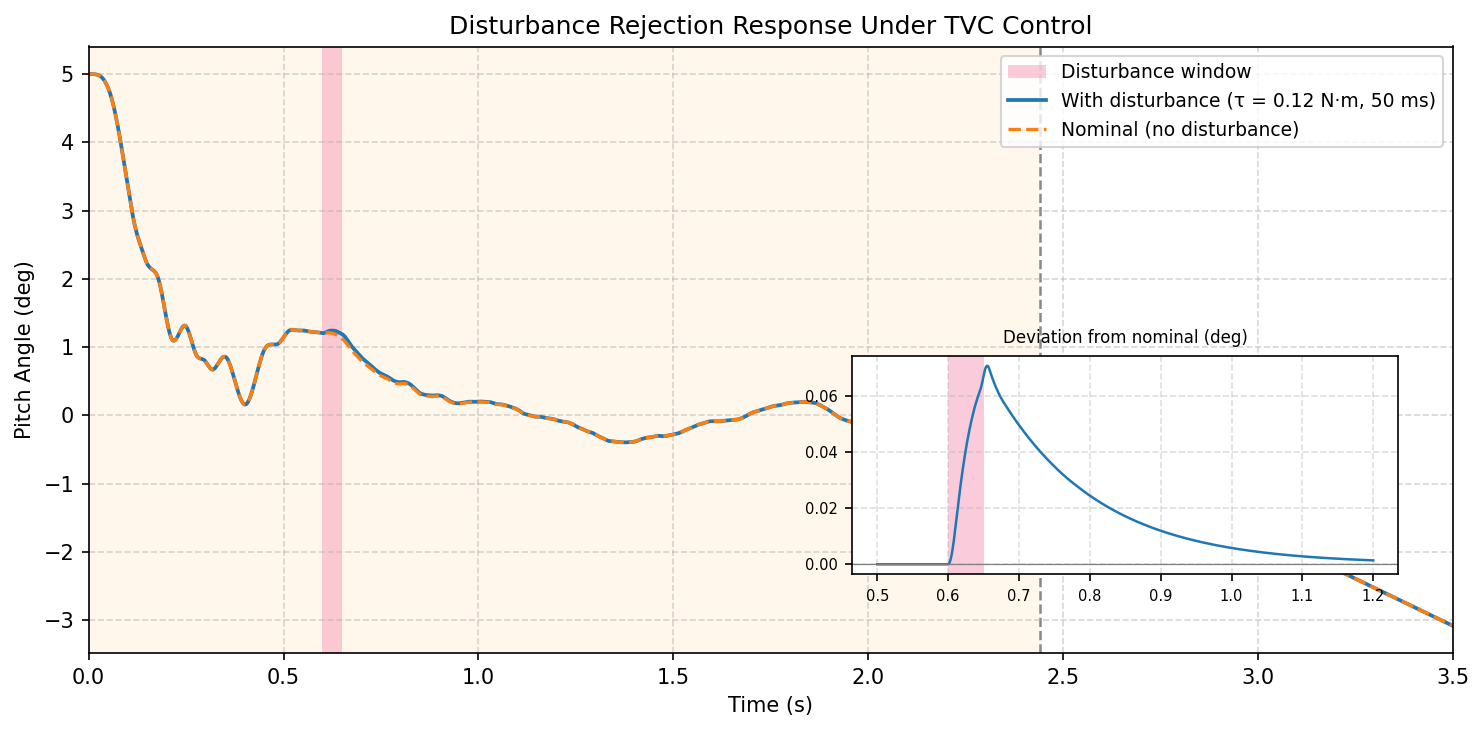
\includegraphics[width=0.85\linewidth]{figures/fig04_disturbance.png}
    \caption{Disturbance Rejection Response Under TVC Control
             ($\tau = 0.12$~N$\cdot$m, 50~ms at $t = 0.6$~s). Disturbance window
             highlighted. Nominal (no-disturbance) trace shown for comparison.}
    \label{fig:disturbance}
\end{figure}

\FloatBarrier

% -----------------------------------------------------------------------
\subsection{Control Effort and Actuator Utilization}
\label{subsec:control_effort}

Figure~\ref{fig:control_effort} shows how the controller converts attitude errors into actuator
movement and confirms that the servo system remains within its limits. In the top panel, a slight
lag between commanded and actual gimbal deflection highlights the servo's rate limiting during the
initial correction. The bottom panel shows that cumulative actuator saturation is confined almost entirely to the initial tip-over correction ($t < 0.06$ s), during which the commanded signal briefly reaches the $\pm10\degree{}$ mechanical limit; the cumulative saturated fraction decays rapidly thereafter and settles at approximately 1.0\% of the total burn. The top panel's slight lag between the commanded signal and the rate-limited actual deflection is the servo physically catching up to this brief initial command. Together these confirm that the PD gains are well-tuned for the MG90S servo: saturation is limited to the brief initial correction rather than persisting throughout the burn, and the system maintains stability without excessive sustained actuator demand.

\begin{figure}[ht]
    \centering
    % IMAGE NEEDED: Export from Python as sections/fig_control_effort.png
    % (2-panel: top = commanded vs. actual gimbal angle with sat. limits; 
    %  bottom = cumulative saturation fraction vs. time)
    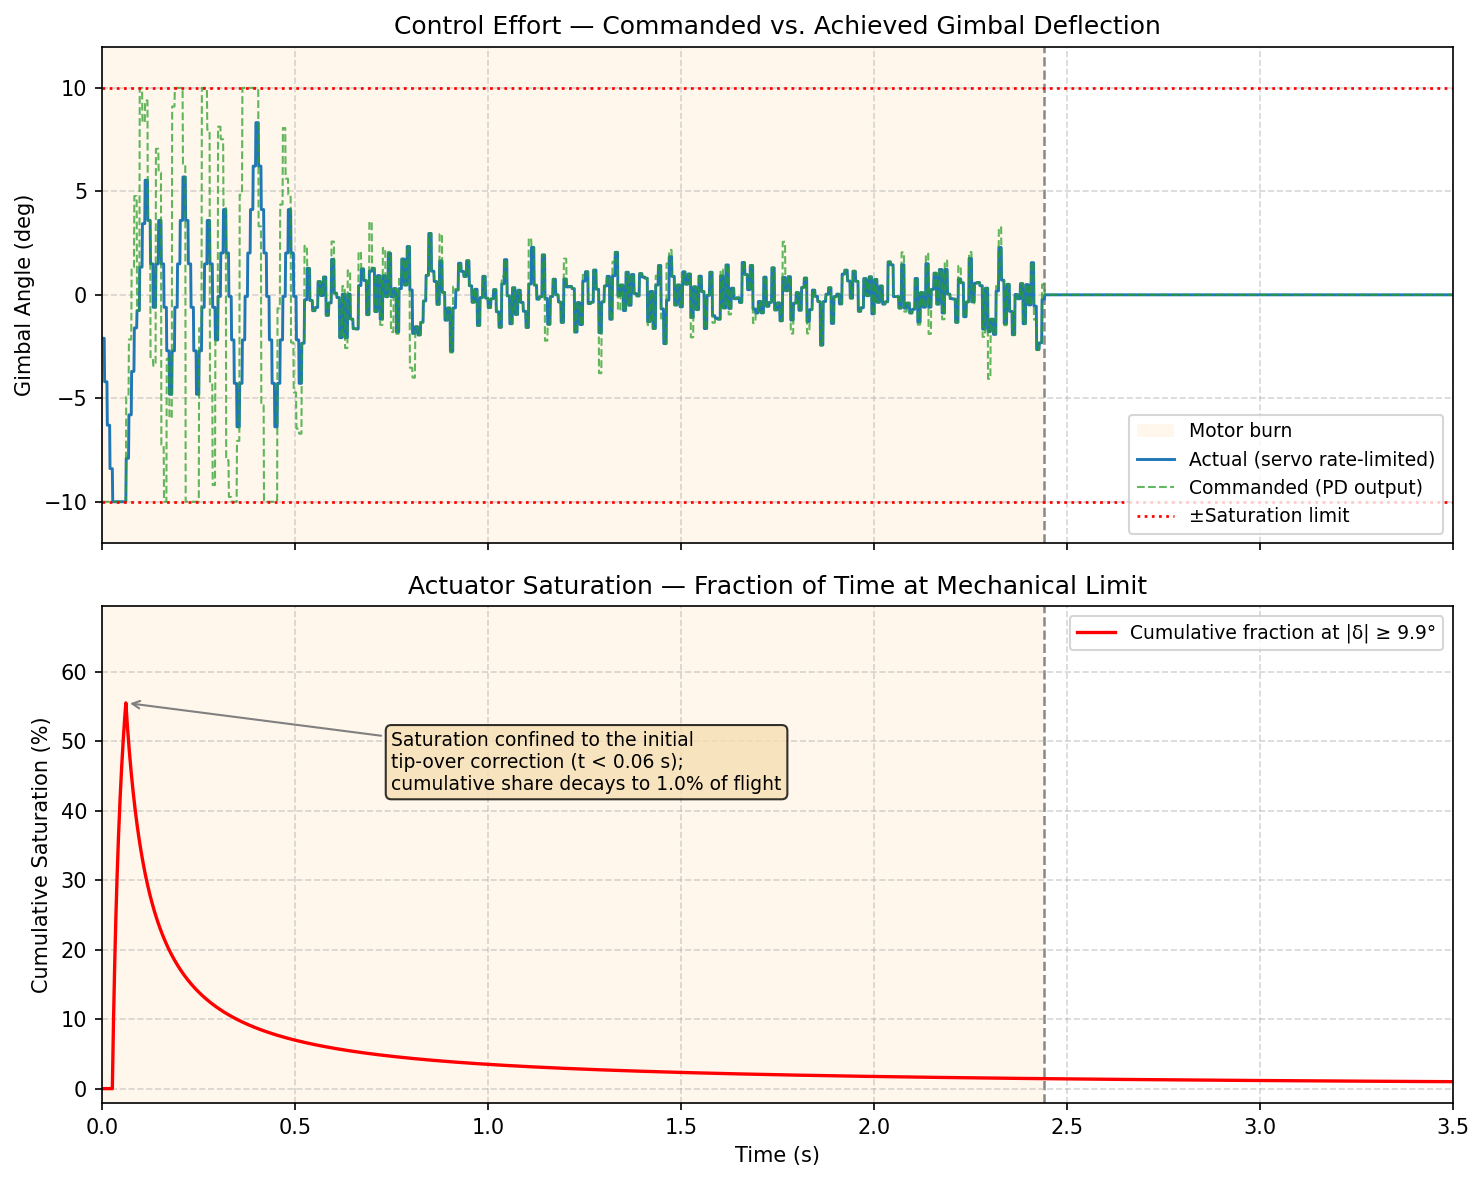
\includegraphics[width=0.85\linewidth]{figures/fig05_control_effort.png}
    \caption{Control Effort --- Commanded vs.\ Achieved Gimbal Deflection (top) and
             Cumulative Actuator Saturation as a fraction of burn time (bottom).
             Saturation is confined to the initial tip-over correction ($t < 0.06$ s) and decays to approximately 1.0\% of the burn thereafter, confirming gains are appropriate for the MG90S servo.}
    \label{fig:control_effort}
\end{figure}

\FloatBarrier

% -----------------------------------------------------------------------
\subsection{Kalman Filter Performance}
\label{subsec:kalman_perf}

Figure~\ref{fig:kalman} isolates the performance of the Kalman filter by comparing the raw
accelerometer signal, the filtered attitude estimate, and the noise-free ground truth across the
full simulation window. During powered flight, the raw accelerometer output is heavily corrupted
by vibration-induced noise, with instantaneous errors exceeding $\pm$4\degree{}. The Kalman
estimate tracks the ground truth closely throughout the burn, suppressing high-frequency noise
while preserving the low-frequency attitude trend. After burnout, the filtered estimate begins to diverge from ground truth: with the control loop disabled and the vehicle in freefall, the accelerometer no longer senses a usable gravity vector, so the filter falls back on gyroscope-only integration, which drifts over time. This is a separate effect from the roll-axis heading drift discussed in Appendix \ref{subsubsec:sensor_limits}, which stems from the MPU-6050's lack of a magnetometer \cite{invensense_mpu6050} and applies only during powered flight. This post-burnout behavior is expected and does not affect the control system, which is disabled after motor shutdown.

\begin{figure}[ht]
    \centering
    % IMAGE NEEDED: Export from Python as sections/fig_kalman_performance.png
    % (ground truth, Kalman estimate, raw accelerometer on same axes;
    %  motor burn shaded; gyro drift post-burnout annotated)
    
\includegraphics[width=0.85\linewidth]{figures/fig08_kalman_performance.png}
    \caption{Kalman Filter Performance --- Noise Rejection vs.\ Raw Measurement
             (MPU-6050 noise model, Section~3.2). The filter suppresses $\pm$4\degree{}
             peak accelerometer noise during powered flight. Gyroscopic drift post-burnout
             is annotated; it does not affect closed-loop stability.}
    \label{fig:kalman}
\end{figure}

\FloatBarrier

% -----------------------------------------------------------------------
\subsection{TVC Corrective Torque Authority}
\label{subsec:torque_authority}

Figure~\ref{fig:torque_authority} plots the maximum corrective torque available from the TVC
system throughout the motor burn, calculated using the relationship from Section~3.4.1:

\[
\tau_{\max} = F_T \cdot r \cdot \sin(\delta_{\max})
\]

The torque peaks at 1.65~N$\cdot$m near maximum thrust and holds steady at approximately
0.5~N$\cdot$m during the sustained burn phase. Since the control authority margin remains
substantial compared to a representative disturbance torque of 0.025~N$\cdot$m, stability is
maintained throughout powered flight. The corrective authority profile mirrors the thrust curve,
as expected from the governing equation. The collapse of available torque at burnout is why the
flight software disables active control immediately after motor shutdown.

\begin{figure}[ht]
    \centering
    % IMAGE NEEDED: Export from Python as sections/fig_torque_authority.png
    % (tau_max vs. time; typical disturbance torque as dashed line;
    %  control authority margin shaded green; insufficient authority region shaded red)
    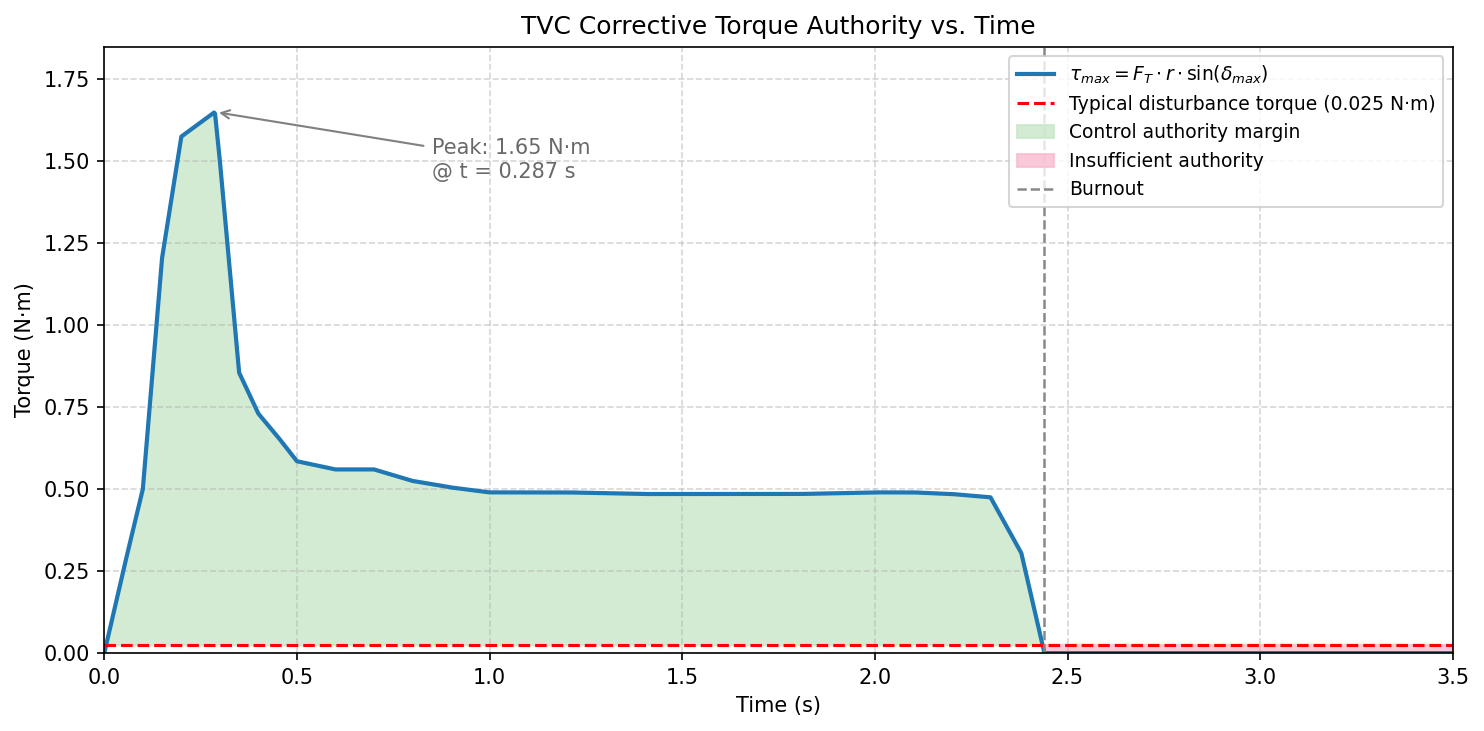
\includegraphics[width=0.85\linewidth]{figures/fig07_control_authority.png}
    \caption{TVC Corrective Torque Authority vs.\ Time
             ($\tau_{\max} = F_T \cdot r \cdot \sin(\delta_{\max})$).
             Green shading: control authority margin above typical disturbance (dashed red).
             Burnout at 2.44~s marked; torque collapses immediately thereafter.}
    \label{fig:torque_authority}
\end{figure}

\FloatBarrier

% -----------------------------------------------------------------------
\subsection{Parametric Sensitivity Analysis}
\label{subsec:sensitivity}

Figure~\ref{fig:sensitivity} analyzes the pitch response sensitivity to three design parameters:
motor thrust scaling, CoM-to-nozzle distance, and maximum gimbal angle. Variations in motor thrust
($\pm$30\%) and CoM-to-nozzle distance ($\pm$20\%) caused negligible changes in recovery
performance, confirming the control architecture's robustness to manufacturing tolerances and
motor lot variation. Maximum gimbal angle had the greatest effect: stable recovery was maintained
even when the limit was reduced to 6\degree{} or 8\degree{}, while increasing it to 12\degree{}
produced a slightly more aggressive initial correction. This confirms that the 10\degree{} design
choice offers adequate authority with a meaningful margin, and that stability is unlikely to be
compromised by minor assembly deviations.

\begin{figure}[ht]
    \centering
    % IMAGE NEEDED: Export from Python as sections/fig_parametric_sensitivity.png
    % (3-panel subplot: (a) thrust variation +-30%, (b) CoM-nozzle distance +-20%,
    %  (c) max gimbal angle 6/8/10/12 deg; all starting from theta_0=5 deg)
    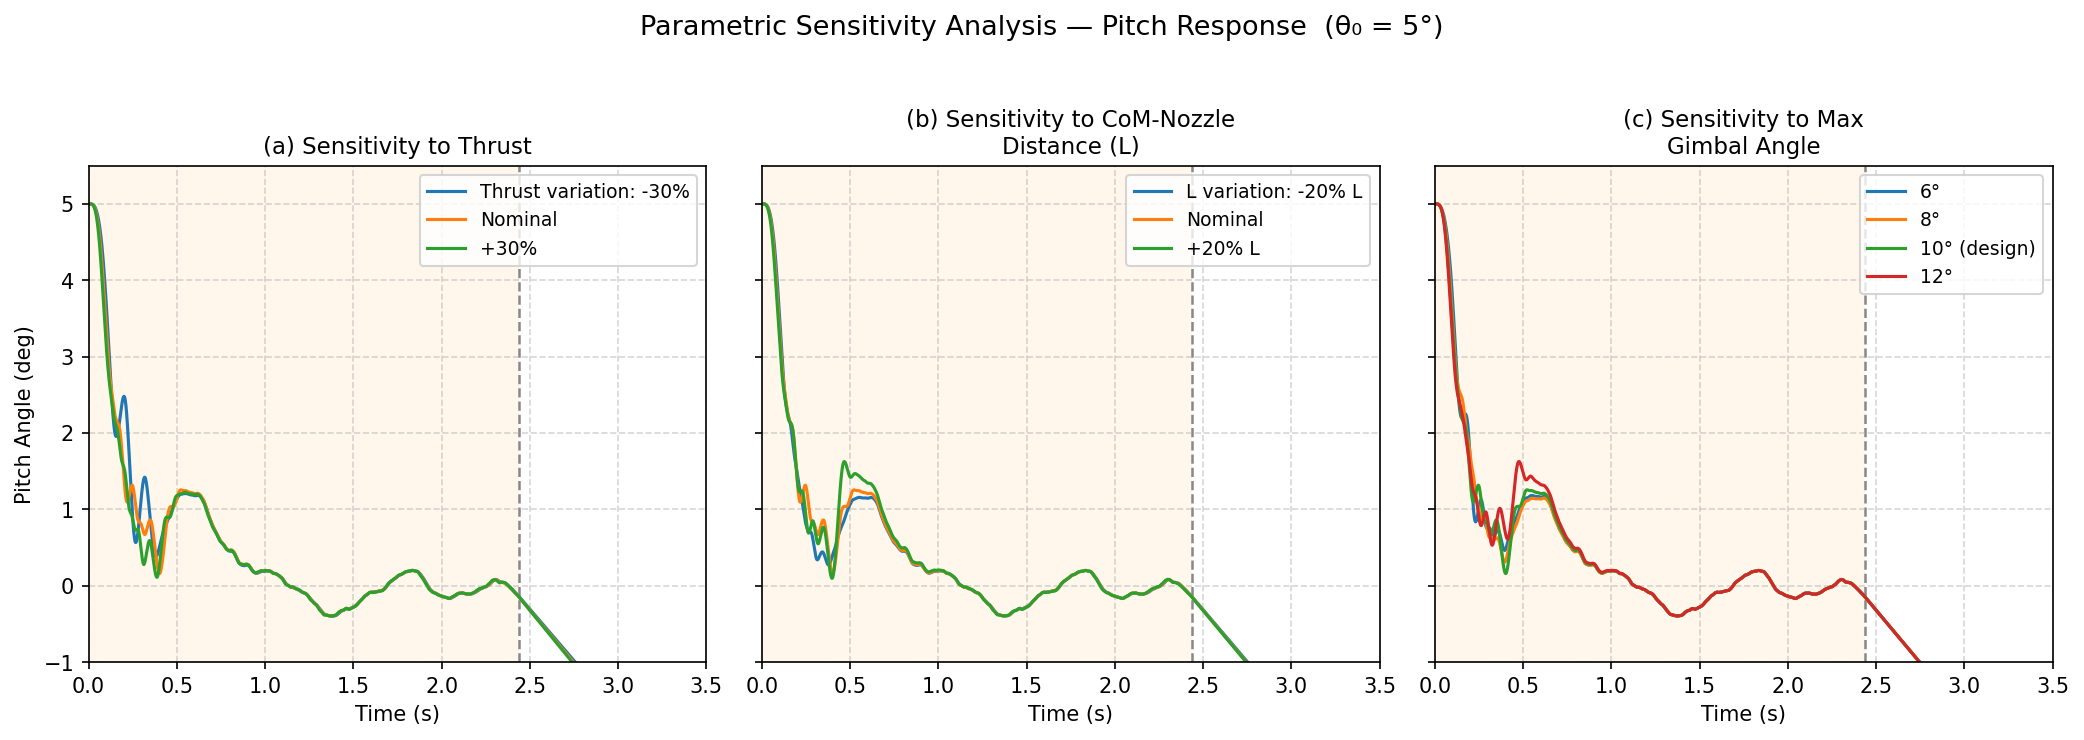
\includegraphics[width=\linewidth]{figures/fig06_sensitivity.png}
    \caption{Parametric Sensitivity Analysis --- Pitch Response ($\theta_0 = 5\degree$).
             (a) Motor thrust variation ($\pm$30\%).
             (b) CoM-to-nozzle distance variation ($\pm$20\%).
             (c) Maximum gimbal angle (6\degree, 8\degree, 10\degree{} design, 12\degree).}
    \label{fig:sensitivity}
\end{figure}

\FloatBarrier

% -----------------------------------------------------------------------
\subsection{Controllability Boundary}
\label{subsec:controllability_boundary}

Figure~\ref{fig:controllability} maps the two-dimensional space of initial pitch angle and initial
angular rate into recoverable and unrecoverable regions, providing a visual representation of the
domain of controllability discussed analytically in Section~3.4. The green region indicates initial
conditions from which the controller successfully recovers the vehicle during powered flight; the
red region represents conditions from which divergence is unavoidable given the gimbal's physical
limits. The boundary occurs at approximately 12\degree{}--15\degree{} of initial pitch angle
depending on initial angular rate, consistent with the theoretical estimate derived in
Section~3.4.2. This figure directly justifies the conservative launch detection thresholds
implemented in Section~4: if the vehicle is tilted beyond this boundary at ignition, no amount of
control effort can recover stable flight.

\begin{figure}[ht]
    \centering
    % IMAGE NEEDED: Export from Python as sections/fig_controllability_boundary.png
    % (2D map: initial pitch angle x-axis, initial angular rate y-axis;
    %  green = recoverable, red = unrecoverable; dashed line at 10 deg gimbal limit)
    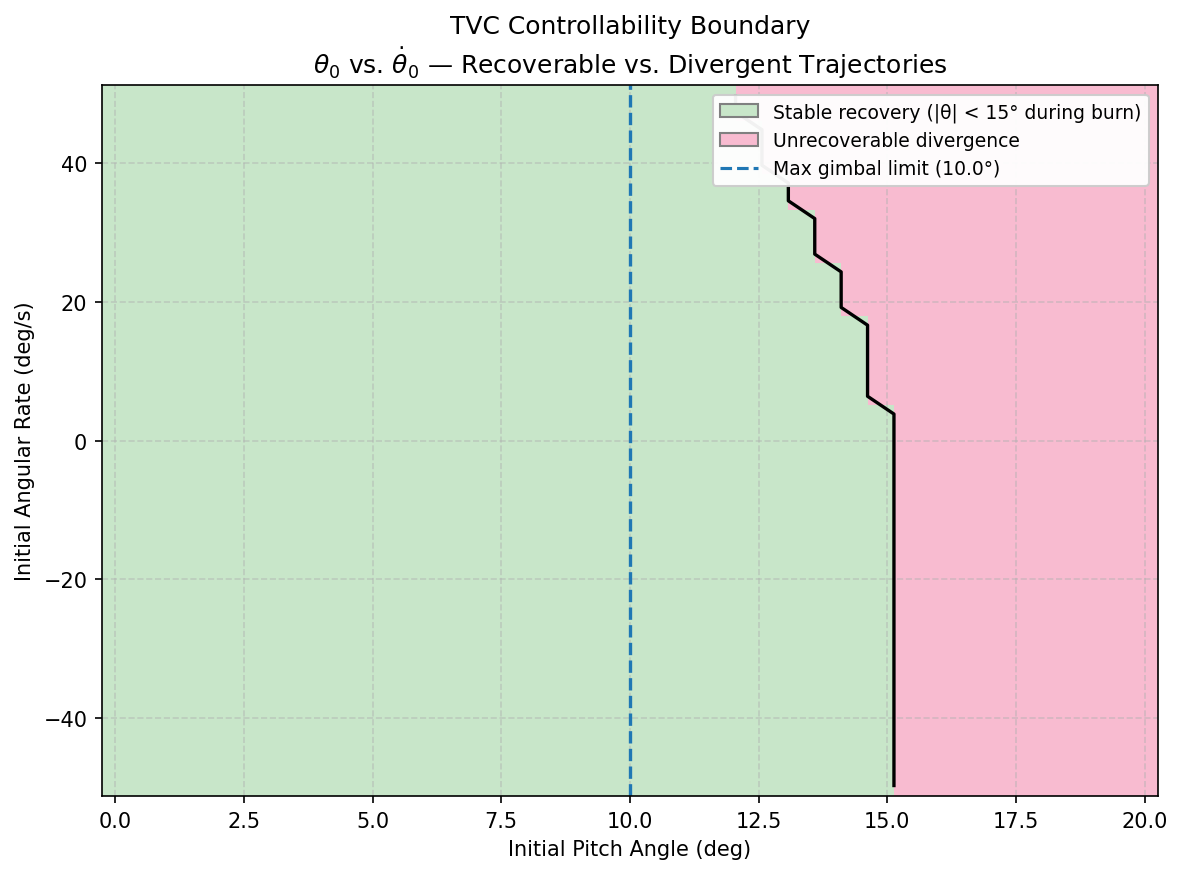
\includegraphics[width=0.85\linewidth]{figures/fig09_stability_boundary.png}
    \caption{TVC Controllability Boundary: $\theta_0$ vs.\ $\dot{\theta}_0$ ---
             Recoverable vs.\ Divergent Trajectories.
             Green: stable recovery ($|\theta| < 15\degree$ during burn).
             Red: unrecoverable divergence.
             Dashed vertical: max gimbal limit (10.0\degree).}
    \label{fig:controllability}
\end{figure}

\FloatBarrier

% -----------------------------------------------------------------------
\subsection{Two-Axis Monte Carlo Simulation}
\label{subsec:monte_carlo}

Figure~\ref{fig:monte_carlo} provides the section's most thorough validation through 100
independent trials. These trials randomized initial pitch and yaw angles (0.5\degree{} to
6\degree{}), scaled thrust by $\pm$8\% to mimic motor manufacturing variance, and included IMU
sensor noise at levels consistent with the MPU-6050 datasheet \cite{invensense_mpu6050}. In every
trial, the rocket recovered successfully during powered flight and maintained stable orientation.
The rapid narrowing of the 5th-to-95th percentile envelope after the initial correction confirms
consistent performance across all input variables. While individual traces diverge after burnout
due to independent gyroscopic drift, the results collectively demonstrate that the control
architecture is robust against realistic launch variability, provided the vehicle begins flight
within the recoverable envelope defined in Section~\ref{subsec:controllability_boundary}.

\begin{figure}[ht]
    \centering
    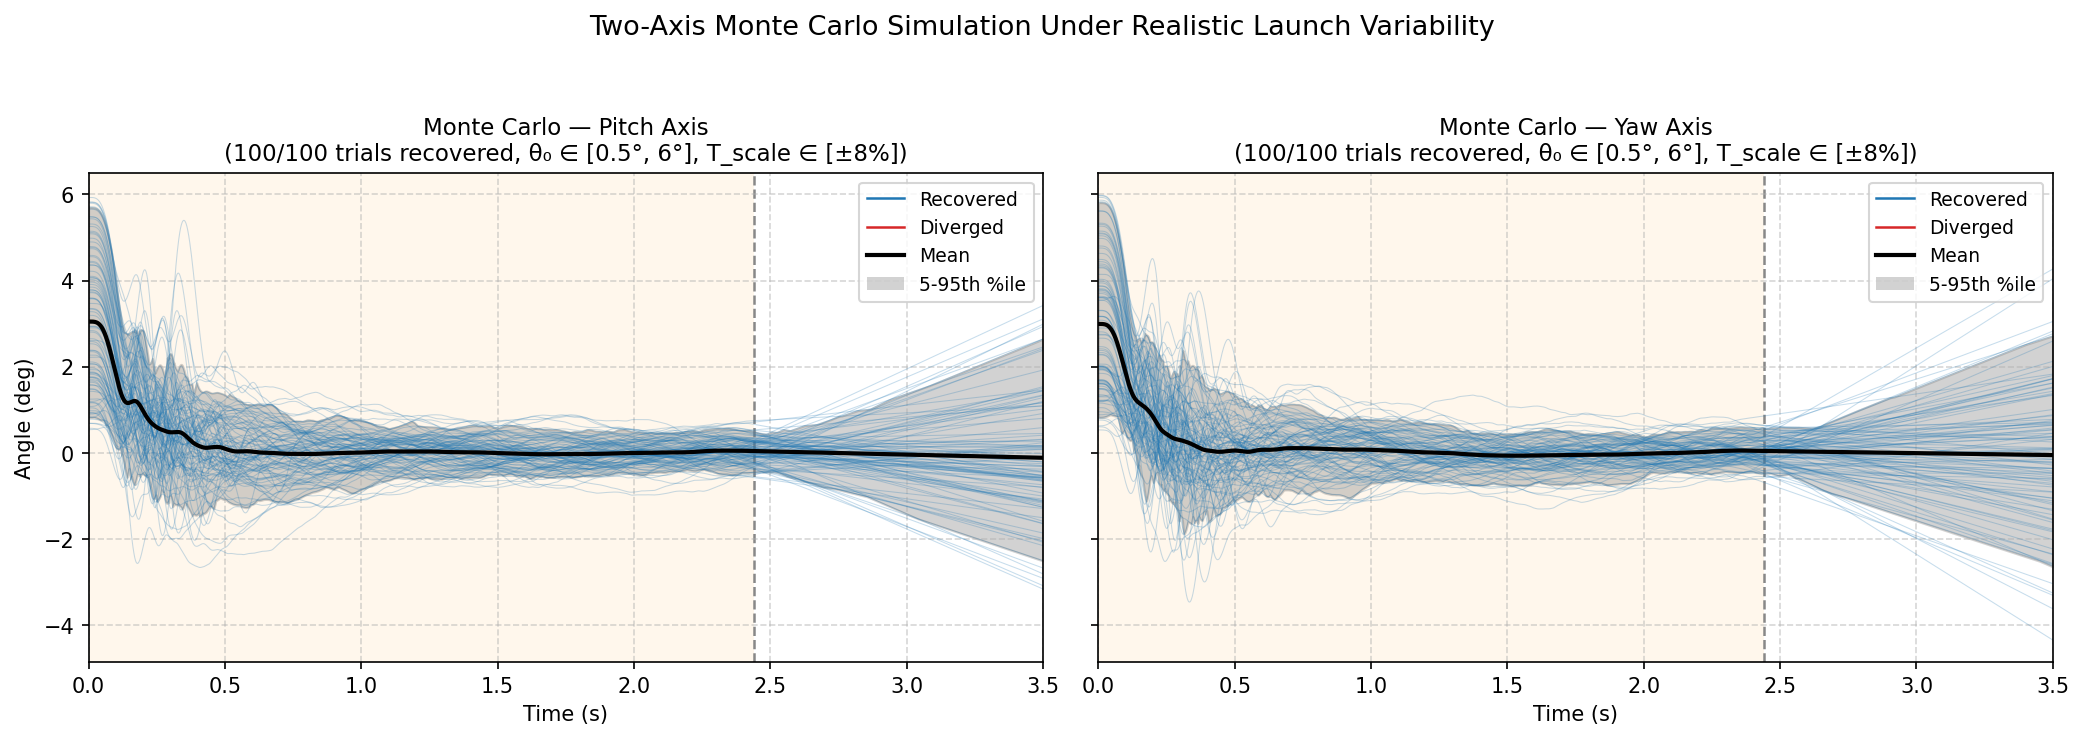
\includegraphics[width=\linewidth]{figures/fig10_monte_carlo.png}
    \caption{Two-Axis Monte Carlo Simulation Under Realistic Launch Variability
             (100 trials; $\theta_0 \in [0.5\degree,\,6\degree]$,
             $T_{\mathrm{scale}} \in [\pm 8\%]$, sensor noise included).
             Pitch (left) and yaw (right) axes shown independently.
             100/100 trials recovered. Mean and 5th--95th percentile envelope shown.}
    \label{fig:monte_carlo}
\end{figure}

\FloatBarrier

% -----------------------------------------------------------------------
\subsection{Discussion of Results and Limitations}
\label{subsec:sim_discussion}

Taken together, the simulations demonstrate consistent closed-loop stability across a wide range
of initial conditions, disturbance magnitudes, and parameter variations. The control system
respects actuator constraints, responds predictably to external inputs, and produces failure modes
that align with the analytical limits derived in Section~3.4 rather than arising from control
instability. The 100\% Monte Carlo recovery rate within the tested envelope provides meaningful
confidence in the architecture's robustness.

The simulations do not capture all real-world effects. Aerodynamic nonlinearities at high angles
of attack, structural vibration and aeroelastic coupling, and launch rail dynamics are not modeled.
Sensor noise models, while representative of the MPU-6050's published characteristics
\cite{invensense_mpu6050}, cannot fully replicate the high-acceleration environment of an actual
motor firing. These results should therefore be interpreted as validation of the system architecture
and control design rather than a guarantee of flight performance. Physical validation using a
2-DOF static test stand---described as future work in Section~7---will provide the next level of
verification.


\begin{table}[h]
\centering
\caption{Summary of Simulation-Based Performance Results}
\label{tab:results-summary}
\begin{tabular}{lc}
\toprule
Metric & Value \\
\midrule
Settling time, baseline 5\degree{} tip-off (Section \ref{subsec:baseline_response}) & $\sim$0.3 s \\
Peak angular deviation, mid-flight disturbance (Section \ref{subsec:disturbance}) & 1.3\degree{} \\
Recovery time, mid-flight disturbance (Section \ref{subsec:disturbance}) & 0.4 s \\
Peak corrective torque, $\tau_{max}$ (Section \ref{subsec:torque_authority}) & 1.65 N$\cdot$m \\
Sustained corrective torque, mid-burn (Section \ref{subsec:torque_authority}) & $\sim$0.5 N$\cdot$m \\
Representative disturbance torque (Section \ref{subsec:torque_authority}) & 0.025 N$\cdot$m \\
Cumulative actuator saturation (Section \ref{subsec:control_effort}) & $\sim$1.0\% of burn \\
Maximum recoverable tilt angle, $\theta_{max}$ (Sections \ref{subsubsec:max_tilt}, \ref{subsec:controllability_boundary}) & 12\degree{}--15\degree{} \\
Kalman filter noise reduction vs.\ raw accelerometer (Section \ref{subsec:kalman}) & 70--80\% \\
Monte Carlo recovery rate, 100 trials (Section \ref{subsec:monte_carlo}) & 100/100 \\
\bottomrule
\end{tabular}
\end{table}

% -----------------------------------------------------------------------
\subsection{Reproducibility and Data Availability}
\label{subsec:reproducibility}

All simulation scripts, parameter files, and plotting code used to generate the figures in this
section are available in the public GitHub repository referenced in Appendix~A.6. Providing access
to these materials allows the results to be independently verified and enables future refinement of
the model.
